\chapter{Main Window}
\label{ch:main}

\section{Overview}

When \software{uPrime} launches you will see a welcome screen. The sidebar on the left is your control panel. All steps are numbered in the order you should use them.

\begin{figure}[htbp]
  \centering
  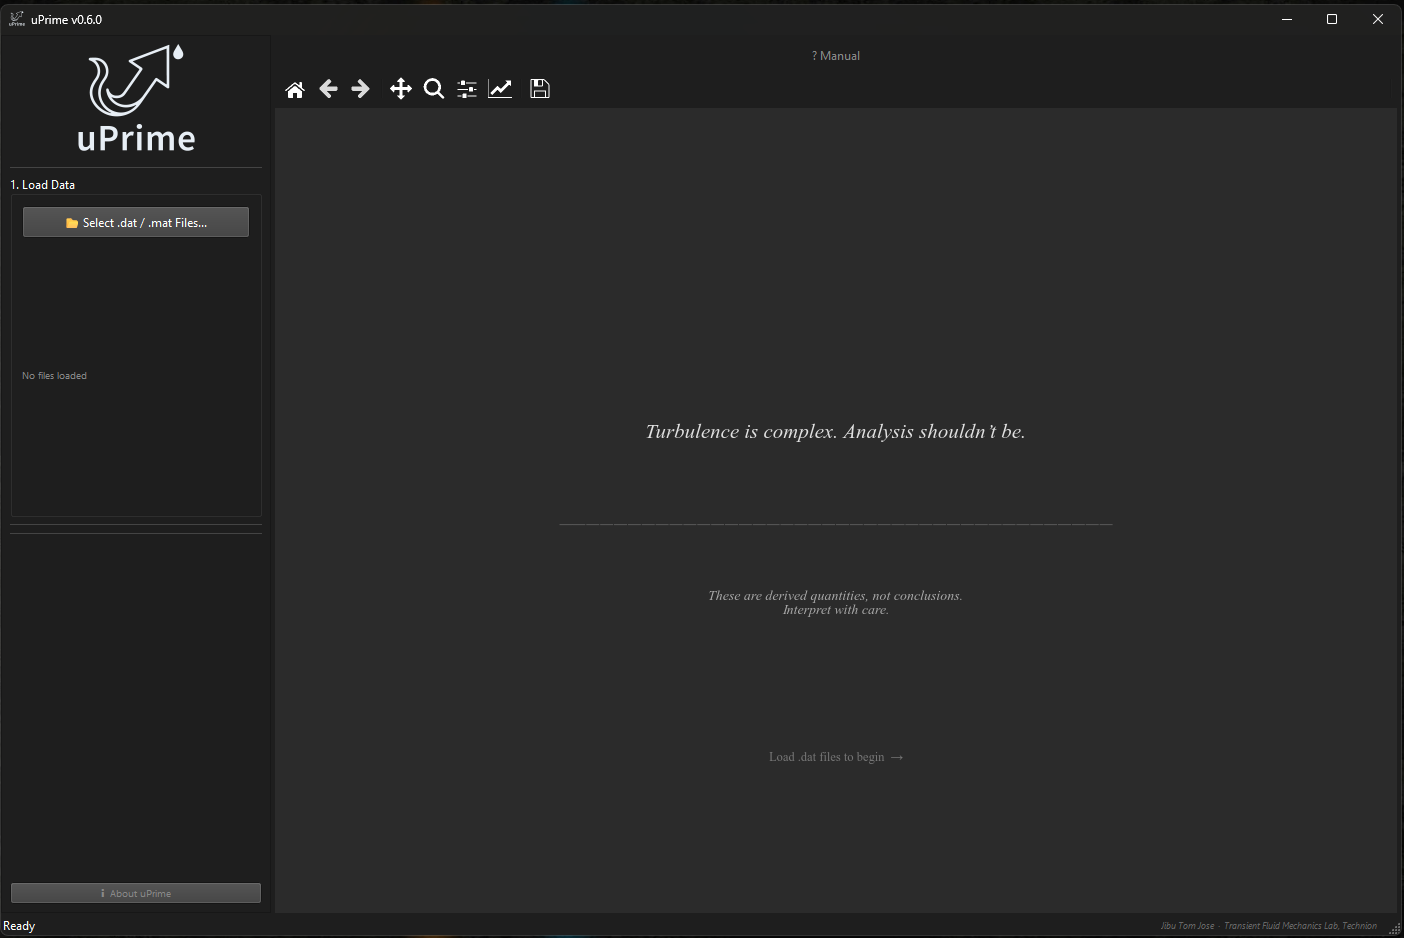
\includegraphics[width=0.92\linewidth]{fig0}
  \caption{\software{uPrime} v0.6.0 welcome screen on launch. The sidebar shows Step~1 (Load Data) only. The \uipth{? Manual} button is visible in the top right. Load \texttt{.dat} or \texttt{.mat} files from the sidebar to begin.}
  \label{fig:welcome}
\end{figure}

\begin{figure}[htbp]
  \centering
  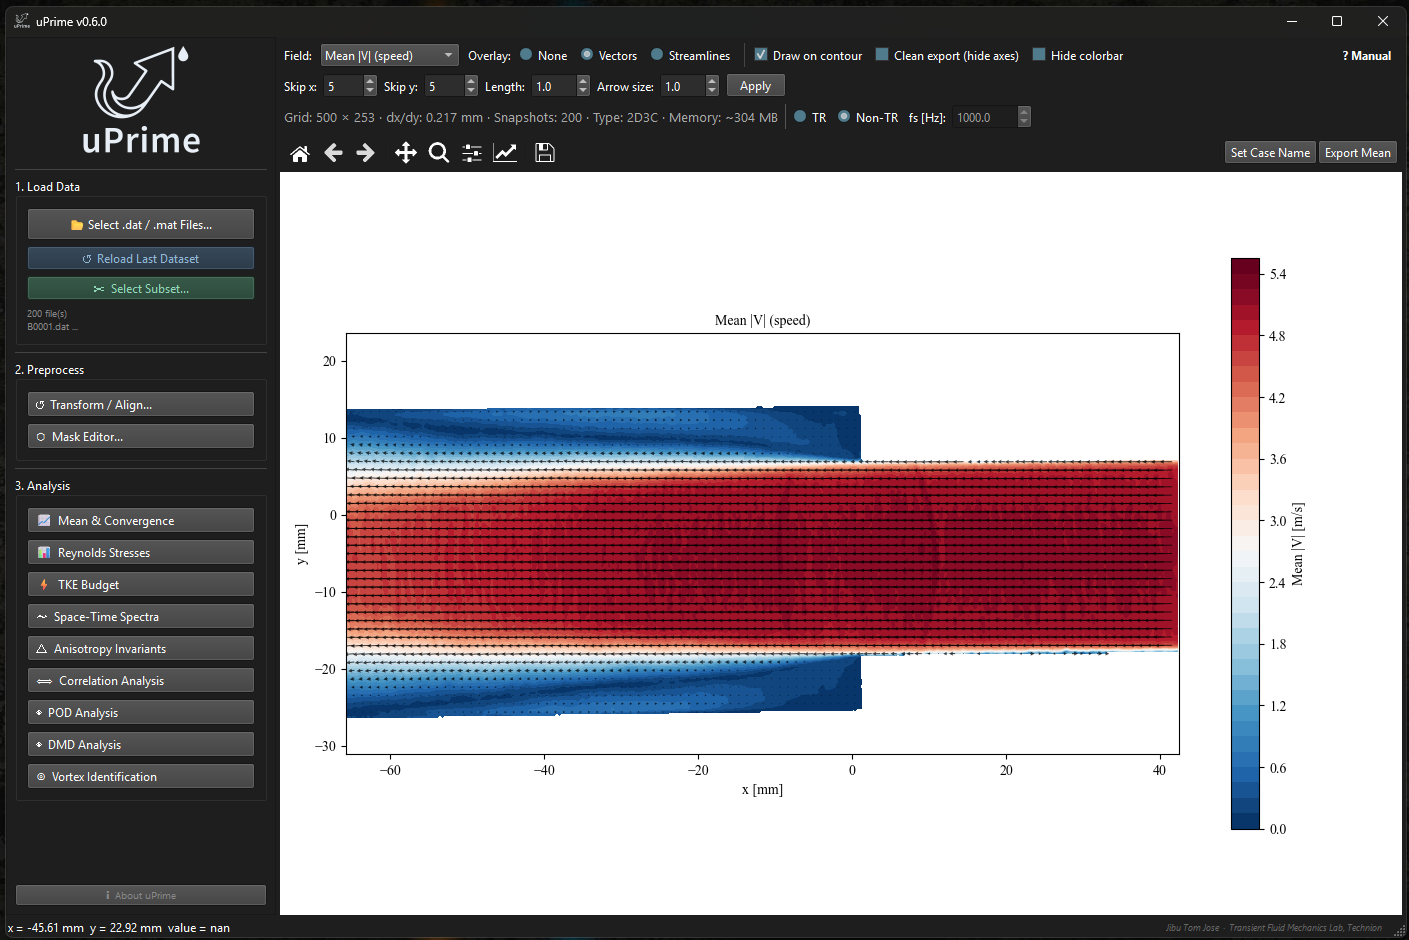
\includegraphics[width=0.85\linewidth]{fig1}
  \caption{Main window after loading a dataset. The Analysis panel lists modules in the recommended order of use, beginning with \uipth{Mean \& Convergence} for verifying statistical convergence before moving to higher-order statistics.}
  \label{fig:main}
\end{figure}

\subsection{Step 1: Load Data}

Click \uipth{Select .dat / .mat Files\ldots} to open a file browser. You can select multiple \texttt{.dat} files (one snapshot each) or a single \texttt{.mat} file (full time series). The file type is auto-detected from the extension.

For \texttt{.dat} loads, a subsampling dialog appears next (see Section~\ref{sec:subsample}). For \texttt{.mat} loads, the variable confirmation dialog appears (see Section~\ref{sec:matformat}).

After loading, the acquisition-type dialog appears. Set \uipth{TR} (time-resolved) or \uipth{Non-TR} and enter the sampling frequency $f_s$ if TR.

\begin{figure}[htbp]
  \centering
  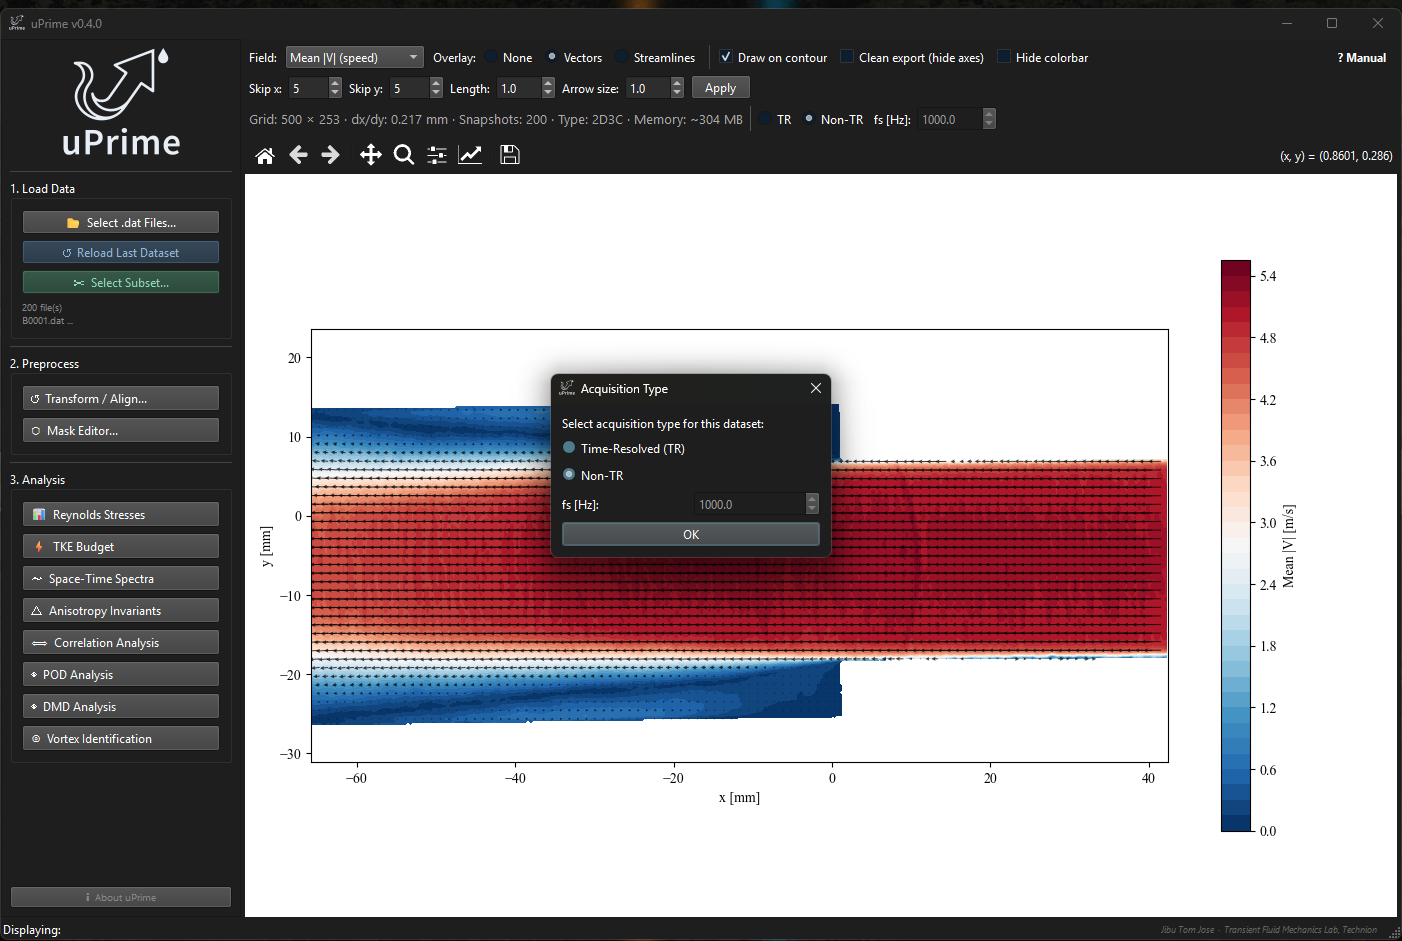
\includegraphics[width=0.85\linewidth]{fig_acqtype}
  \caption{Acquisition type dialog shown automatically after each data load. Select TR and enter $f_s$ to enable temporal analysis modules. The $f_s$ spinbox is greyed out when Non-TR is selected.}
  \label{fig:acqtype}
\end{figure}

\subsection{Step 2: Preprocess}

Click \uipth{Transform / Align\ldots} to open the coordinate correction tool. This is where you fix camera tilt, shift the coordinate origin, and optionally mirror the dataset. \textbf{Always do this before running any analysis.} Full details are in Chapter~\ref{ch:transform}.

Click \uipth{Mask Editor\ldots} to draw additional spatial masks over regions you want to exclude from analysis (e.g.\ reflections, shadows, or wall regions not detected by the DaVis isValid flag). Masks are non-destructive: the raw velocity data is never modified. Toggling a mask on or off does not require reloading.

\begin{figure}[htbp]
  \centering
  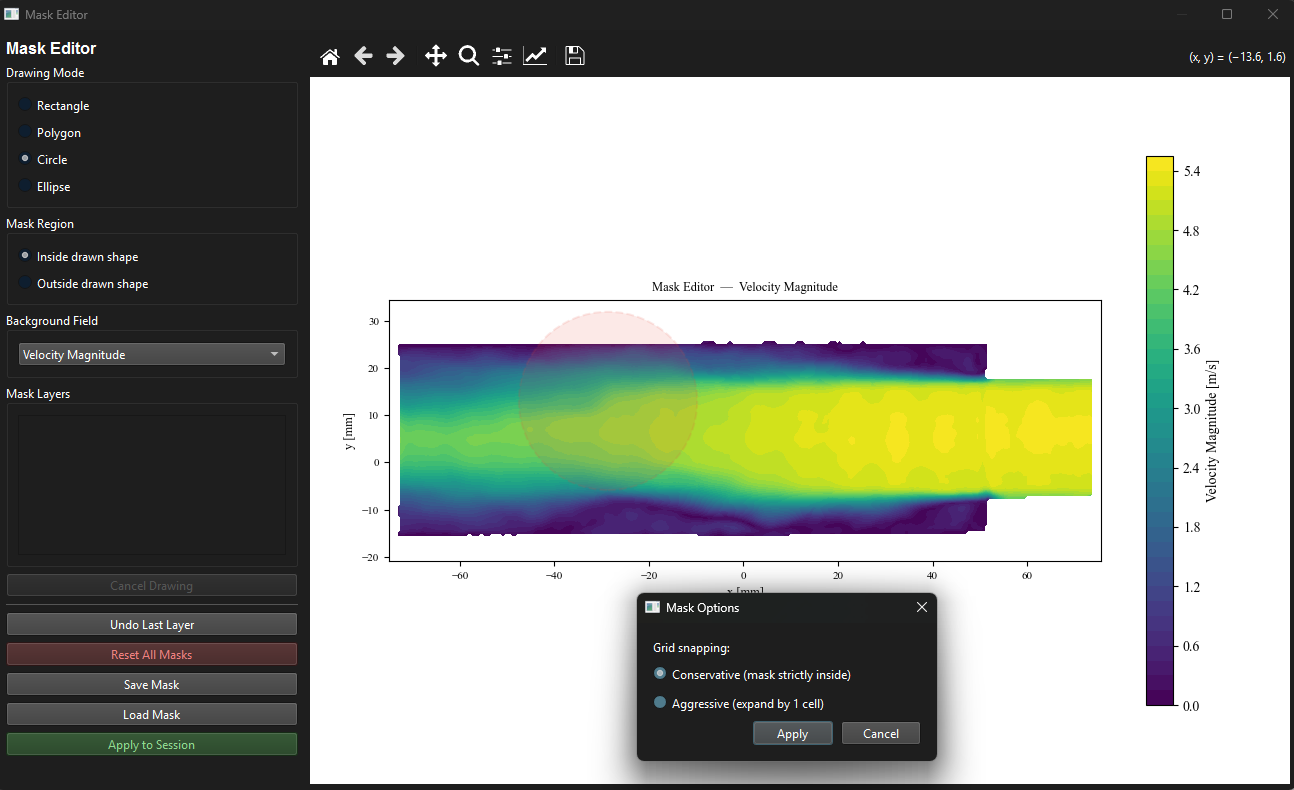
\includegraphics[width=0.92\linewidth]{fig_maskeditor}
  \caption{Mask Editor window. The user is drawing a polygon (red) over a region to exclude. Drawing modes include Rectangle, Polygon, Circle, and Ellipse. The mask can be applied inside or outside the drawn shape. Multiple layers can be stacked and each can be undone independently.}
  \label{fig:maskeditor}
\end{figure}

\begin{figure}[htbp]
  \centering
  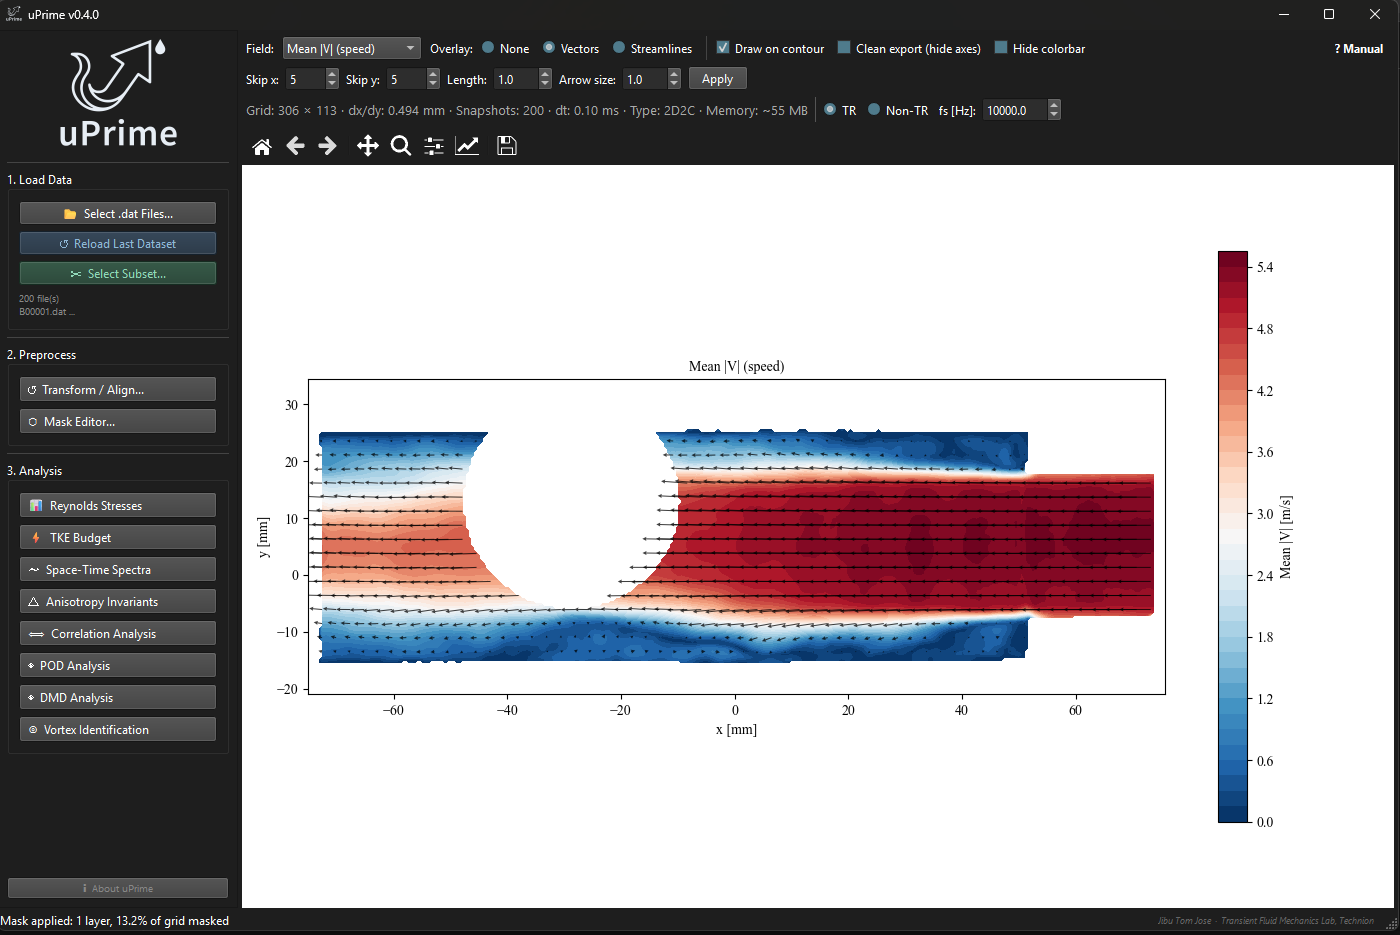
\includegraphics[width=0.92\linewidth]{fig_mask_main}
  \caption{Main window after applying a drawn mask. The masked region is shown in white. The status bar at the bottom reports the number of mask layers and the fraction of the grid that is masked.}
  \label{fig:maskmain}
\end{figure}

\subsection{Step 3: Analysis}

Click any analysis button to open that module in its own window. Multiple analysis windows can be open at the same time and can be compared side by side. The recommended starting point is \uipth{Mean \& Convergence} (Chapter~\ref{ch:meanconv}); from there proceed to Reynolds stresses, TKE budget, and the higher-order modules as appropriate.

All heavy computations (POD, DMD, TKE budget, correlation, vortex identification) run in a background thread so the main window remains fully responsive during computation. A progress indicator appears below the compute button while the calculation is in progress.

\section{Acquisition type and sampling frequency}

The acquisition type and sampling frequency $f_s$ are set in the dataset info ribbon at the top of the main window, immediately below the field options strip. A dialog to set these values also appears automatically after each data load.

\begin{itemize}[leftmargin=1.5em]
  \item \uipth{TR}: snapshots are acquired at a fixed rate. Enter $f_s$ in Hz (enabled only for TR). Temporal analyzes (temporal spectra, temporal correlation, POD temporal coefficients, DMD) become available.
  \item \uipth{Non-TR}: snapshots are statistically independent (e.g.\ double-frame PIV). Temporal analyzes are greyed out.
\end{itemize}

\begin{warnbox}
Set the correct acquisition type and $f_s$ before opening any analysis window. Analysis windows read these settings when they open.
\end{warnbox}

\section{Dataset info ribbon}
\label{sec:datasetinfo}

A compact info strip appears just below the options strip after loading:

\begin{center}
\texttt{Grid: 507\,$\times$\,248 $\cdot$ dx/dy: 0.165\,mm $\cdot$ Snapshots: 2000 $\cdot$ dt: 0.10\,ms $\cdot$ Type: 2D2C $\cdot$ Memory: \textasciitilde{}2012\,MB}
\end{center}

\begin{itemize}[leftmargin=1.5em]
  \item \textbf{Grid}: number of velocity vectors in $x$ and $y$.
  \item \textbf{dx / dy}: spatial resolution in mm. For \texttt{.mat} files this is estimated from the coordinate arrays using the median of differences (robust to small rounding at the edges). A non-uniform grid (more than 1\% variation in spacing) triggers a status-bar warning, since FFT and Welch spectra assume uniform grids.
  \item \textbf{Snapshots}: how many snapshots are currently active (reflects subsampling).
  \item \textbf{dt}: time between frames in milliseconds (TR data only; updates if $f_s$ or stride changes).
  \item \textbf{Type}: \texttt{2D2C} for planar PIV; \texttt{2D3C} for stereo PIV with $W$.
  \item \textbf{Memory}: estimated RAM used by the velocity arrays. For datasets exceeding 4\,GB, this reflects the size of the memory-mapped file on disk rather than physical RAM consumed (see Section~\ref{sec:subsample}).
\end{itemize}

\section{Field viewer}

The right panel shows the selected velocity field as a filled contour plot with optional velocity vectors.

\subsection{Display controls}

\begin{table}[htbp]
\centering
\caption{Field viewer display controls.}
\begin{tabular}{lp{9cm}}
\toprule
\textbf{Control} & \textbf{Description} \\
\midrule
Field         & Quantity to show: Mean U/V/W, speed $|V|$, vorticity, Std(U), Std(V) \\
Overlay       & None, Vectors, or Streamlines \\
Draw on contour & When checked, overlays the selected overlay on the filled contour \\
Clean export  & Hides all axis labels, tick marks, and the plot title for a clean exported image \\
Hide colorbar & Removes the colorbar from the plot \\
? Manual      & Opens the user manual PDF \\
\bottomrule
\end{tabular}
\end{table}

\subsection{Streamlines}

Streamlines trace the instantaneous mean velocity field and give a cleaner visual impression of the flow topology than arrow vectors, especially in regions with complex recirculation.

\begin{stepbox}
\begin{enumerate}[leftmargin=1.5em, topsep=2pt]
  \item Set \uipth{Overlay} to \uipth{Streamlines}.
  \item The vector ribbon appears. Left-click and drag on the field to draw a rake seed line. Multiple rakes can be drawn cumulatively.
  \item Adjust \uipth{Length}, color, and line width in the ribbon.
  \item Click \uipth{Apply} to redraw.
  \item Click \uipth{Reset} in the ribbon to clear all seed rakes and start over.
\end{enumerate}
\end{stepbox}

\begin{notebox}
Streamlines are drawn from the mean velocity field only. They do not reflect instantaneous snapshot structure.
\end{notebox}

\subsection{Toolbar}

\begin{table}[htbp]
\centering
\caption{Toolbar button functions.}
\begin{tabular}{ll}
\toprule
\textbf{Button} & \textbf{Function} \\
\midrule
Home           & Resets the view to the original limits, regardless of zoom history \\
Back / Forward & Step through zoom history \\
Pan            & Click and drag to pan the view \\
Zoom           & Click and drag a rectangle to zoom in \\
Save           & Save the figure as PNG (300 DPI), PDF, or SVG \\
\bottomrule
\end{tabular}
\end{table}

\subsection{Saving figures}

Click the Save button in the toolbar. PNG is saved at 300\,DPI. PDF and SVG use vector graphics; all text is saved as editable text and can be restyled in Adobe Illustrator or Inkscape.

\begin{tipbox}
For publication figures: (1) enable \uipth{Clean export} to hide axes, (2) enable \uipth{Hide colorbar} if not needed, (3) save as SVG and open in Illustrator to set your journal's font and size requirements.
\end{tipbox}

\section{Export menu}

The \uipth{Export} menu in the menu bar provides one-click export of the time-averaged mean field as a Tecplot ASCII \texttt{.dat} file. The exported file contains $\langle U \rangle$, $\langle V \rangle$, $|V|$, and (for stereo data) $\langle W \rangle$ on the original grid, ready for use in CFD validation, plotting in Tecplot, or import into other PIV tools.

\begin{figure}[htbp]
  \centering
  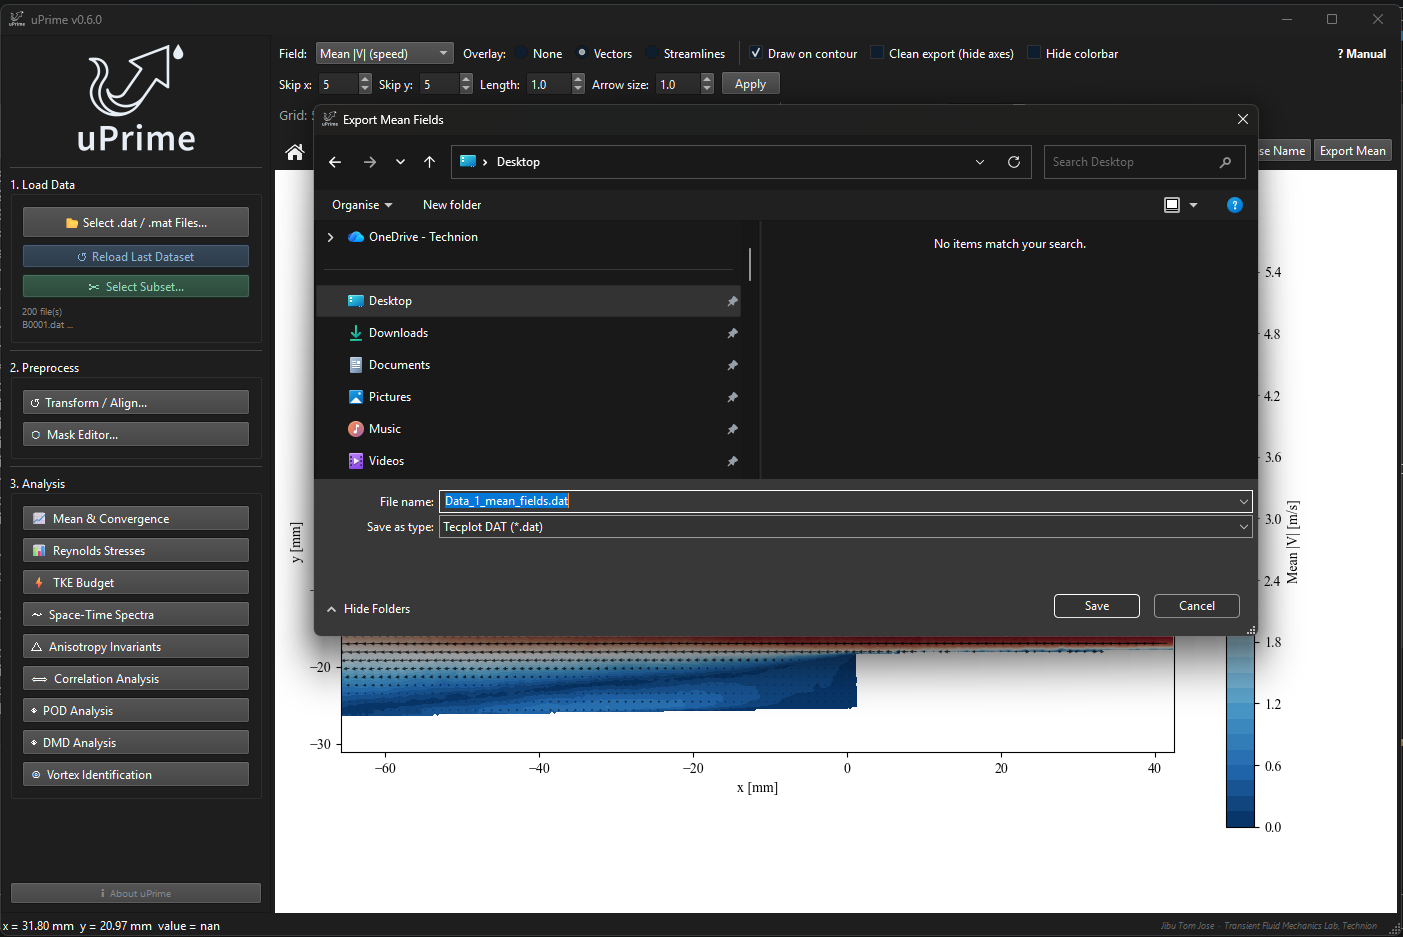
\includegraphics[width=0.6\linewidth]{fig_export_menu}
  \caption{Main window \uipth{Export} menu showing the Tecplot ASCII mean field export option.}
  \label{fig:exportmenu}
\end{figure}

\section{Snapshot subsampling and large dataset handling}
\label{sec:subsample}

A subsampling dialog appears whenever \texttt{.dat} files are selected, giving you control over how many snapshots to load. The same controls (start, end, step) are available inside the \texttt{.mat} variable confirmation dialog (Section~\ref{sec:matformat}).

\begin{itemize}[leftmargin=1.5em]
  \item \textbf{Load all}: load every file in the selection.
  \item \textbf{Stride}: load every $K$-th snapshot. Stride~5 on a 10,000-snapshot dataset gives 2000 samples, which is sufficient for mean fields, Reynolds stresses, and correlations.
  \item \textbf{Limit}: load only the first $N$ snapshots.
\end{itemize}

The dialog shows the estimated snapshot count and memory usage, updating live as you change the options.

After loading, click \uipth{Select Subset\ldots} to adjust the active snapshot range without re-reading from disk.

\begin{tipbox}
For 10,000+ snapshot datasets, start with Stride~5 ($\sim$2000 samples). Mean fields and Reynolds stresses converge well at this level. Run POD and DMD on the full set once you know what you are looking for. Use the \uipth{Mean \& Convergence} module (Chapter~\ref{ch:meanconv}) to verify whether your subsample is sufficient.
\end{tipbox}

\subsection{Large dataset handling (datasets exceeding 4\,GB)}

When the estimated dataset size after subsampling exceeds 4\,GB, \software{uPrime} automatically switches to a \textbf{memory-mapped} loading strategy. Instead of loading all velocity data into RAM, \software{uPrime} writes the data to a temporary binary file on your system's temp drive (typically \texttt{C:\textbackslash Users\textbackslash \textit{username}\textbackslash AppData\textbackslash Local\textbackslash Temp}) and accesses it as needed. The actual path is shown in the warning label inside the subsampling dialog.

\begin{notebox}
Memory-mapped loading requires free disk space on your system temp drive equal to the dataset size. For a 10,000-snapshot 2D2C dataset at a typical grid size, this is approximately 10\,GB. The temporary file is deleted automatically when \software{uPrime} closes normally.
\end{notebox}

\begin{warnbox}
If \software{uPrime} crashes or is forcibly closed, the temporary file may not be deleted. In that case, navigate to your system temp folder and delete any files named \texttt{uprime\_memmap\_*.bin} manually to recover disk space.
\end{warnbox}

The key practical differences when memory-mapped loading is active:

\begin{itemize}[leftmargin=1.5em]
  \item \textbf{Initial load is slower}: \software{uPrime} writes the full dataset to disk before opening it. On a fast SSD, expect 30--90 seconds for a 10\,GB dataset in addition to the normal file reading time.
  \item \textbf{All analysis works normally}: POD, DMD, TKE budget, spectra, correlation, and vortex identification all function identically. Memory-mapped arrays behave like regular numpy arrays.
  \item \textbf{RAM usage is reduced}: only the pages of data currently being accessed are held in RAM. The operating system manages this automatically.
  \item \textbf{Do not load from external drives}: if your \texttt{.dat} files are on an external HDD, copy them to a local drive first. Reading from an external drive while also writing the memory-mapped cache to the temp drive simultaneously will be very slow.
\end{itemize}

\begin{tipbox}
If your system temp drive (usually C:) does not have enough free space, use Stride subsampling to reduce the dataset to under 4\,GB before loading. For example, Stride~3 on a 10,000-snapshot dataset gives $\sim$3333 snapshots ($\sim$3.3\,GB for a typical 2D2C grid), which stays below the threshold and loads entirely into RAM.
\end{tipbox}

% ============================= CHAPTER 3 ==============================
